\documentclass[a4paper]{article}

\usepackage[romanian]{babel}
\usepackage{amsmath}
\usepackage{csquotes}
\usepackage{fontspec}
\usepackage{graphicx}

\usepackage{minted}
\usemintedstyle{emacs}

\usepackage[backend=biber]{biblatex}
\addbibresource{main.bib}

\usepackage{geometry}
\geometry{
  top=3.5cm,
  bottom=3.5cm,
  left=3.5cm,
  right=3.5cm,
}

\usepackage{hyperref}
\hypersetup{
    colorlinks,
    citecolor=black,
    filecolor=black,
    linkcolor=black,
    urlcolor=black
}

\usepackage{tikz}
\usetikzlibrary{decorations.pathreplacing}

\newcommand\MemoryLayout[1]{
  \begin{tikzpicture}[scale=0.3]
     \foreach \pt/\lbl/\col/\lab [remember=\pt as \tp (initially 0)] in {#1} {
       \draw[thick](\pt,0)--++(0,3)node[above]{$\lbl$};
       \foreach \a [parse=true] in {\tp,...,\pt-1} {
          \draw[fill=\col](\a,0) rectangle ++(1,2);
       }
       \if\lab\relax\relax\else
         \draw[thick,decorate, decoration={brace,amplitude=4mm}]
            (\pt,-0.2)--node[below=4mm]{\lab} (\tp,-0.2);
       \fi
     }
     \draw[thick](0,0)--++(0,3)node[above]{$0$};
  \end{tikzpicture}
}

\begin{document}
\begin{titlepage}
	\begin{center}
		\Large Proiect pentru obținerea atestării profesionale în informatică
		\vfill
		\LARGE\textbf{Octarou: Interpretor pentru limbajul de programare CHIP-8}

		\vspace{8pt}
		\Large Nicolas-Ștefan Bratoveanu \\
		\large Prof. coordonator Mihaela Stan

		\vfill
		\Large
		Colegiul Național „Vasile Alecsandri” Galați \\
		2023-2024
	\end{center}
\end{titlepage}

\tableofcontents
\newpage

\section{Introducere}
\subsection{Contextualizare}
\textit{Octarou} este un interpretor pentru limbajul de programare CHIP-8. Acesta este un limbaj de programare interpretat, dezvoltat
de către Joseph Weisbecker în 1977 pentru sisteme bazate pe microprocesorul RCA 1802. A fost inițial utilizată pe computerele COSMAC VIP și Telmac
1800. Limbajul a fost creat cu scopul de a permite dezvoltarea mult mai ușoară a jocurilor video pe aceste platforme, permițând utilizarea unor
instrucțiuni hexazecimale, în locul instrucțiunilor native \cite{langhoff}. Spre sfârșitul anilor '70, în spatele acestui limbaj se formase o comunitate activă
de dezvoltatori și utilizatori, care a luat naștere odată cu buletinul informativ \textit{VIPer} al revistei \textit{ARESCO}, ale cărei prime
ediții au dezvăluit codul pentru interpretorul original de CHIP-8.

CHIP-8 s-a răspândit pe alte platforme, precum computerele australiene DREAM 6800, ETI-660 și MicroBee, computerul finlandez menționat mai devreme,
Telmac 1800 și computerul canadian ACE VDU \cite{langhoff}.

Ulterior, au apărut interpretoare derivate și extensii la limbajul original, folosite, spre exemplu, pe calculatoare grafice (CHIP-48, SUPER-CHIP
pentru calculatoarele HP-48 \cite{langhoff}). Aceste dispozitive aparțineau perioadei de după anii '80 și aveau, de regulă, mult mai multă putere de procesare
decât microcomputerele din deceniul precedent, cum ar fi COSMAC VIP-ul.

\subsection{Motivația alegerii temei}
La nivel de suprafață, alegerea acestei teme poate părea (cel puțin) dubioasă. Cu toate că este, într-adevăr, o temă destul de obscură, consider
că este extrem de valoroasă. Astfel de proiecte au valoare din punct de vedere al istoriei calculatoarelor, precum și în cadrul fenomenului de
„retro-computing”. Mai mult decât atât, CHIP-8, în mod specific, are o valoare educațională deosebită, întrucât implementarea unui astfel de
sistem este adesea recomandată ca prim pas în lumea dezvoltării de emulatoare \cite{langhoff}.

\section{Mediul de dezvoltare}
\subsection{Rust}
Am ales Rust ca limbaj principal de dezvoltare pentru acest proiect. Rust este un limbaj de programare general, multi-paradigmă, care pune accent
pe siguranță, eficiență și paralelism. Este utilizat în numeroase situații, de la programarea sistemelor, la dezvoltarea de aplicații grafice, dezvoltarea
web sau a sistemelor integrate.

Performanța și eficiența se datorează absenței unui runtime și a unui \textit{garbage collector}. Siguranța memoriei este asigurată de către sistemul
de tipuri bogat și de modelul de \textit{ownership}, care permit eliminarea a numeroase tipuri de buguri în stagiul de compilare \cite{rsorg}. Modelul
de \textit{ownership} impune niște reguli privitoare la deținători \cite[Cap.~4.1]{rustbook}:
\begin{itemize}
	\item Orice valoare are un deținător (\textit{owner}).
	\item Nu poate exista decât un deținător la un moment dat.
	\item Când deținătorul iese din scope, valoarea este eliberată.
\end{itemize}
și la utilizarea referințelor \cite[Cap.~4.2]{rustbook}:
\begin{itemize}
	\item Referințele sunt mereu valide.
	\item La un moment dat, pot exista fie mai multe referințe imuabile, fie o singură referință muabilă, dar niciodată ambele.
\end{itemize}

Sistemul de tipuri este extrem de puternic și permite modelarea stării unei aplicații în moduri idiomatice, prin utilizarea tipurilor
pentru a impune invariantele. Spre exemplu, considerăm tipul de date din Listing~\ref{listing:nonzerou8}. Invarianta acestuia este
că valoarea pe care o memorează este diferită de 0. Acest lucru este reprezentat direct în sistemul de tipuri prin utilizarea
\texttt{Option<T>} (echivalent cu \texttt{Maybe a} din Haskell sau \texttt{std::optional<T>} din C++17), un tip polimorfic utilizat
pentru a încapsula o valoare sau \textit{absența acesteia}. Dacă valoarea pe care o primește constructorul \texttt{new} este nulă,
acesta va întoarce valoarea \texttt{None}, pe care apelatorul este forțat să o gestioneze.

\begin{listing}
	\inputminted{rust}{codeblocks/nonzerou8.rs}
	\caption{Exemplu de structură cu invariantă simplă}
	\label{listing:nonzerou8}
\end{listing}

Dacă se încearcă utilizarea valorii de tip \texttt{Option<u8>} ca atare, se obține o eroare de compilare.

\begin{minted}{rust}
let a = NonZeroU8::new(0);
println!("{:?}", a + 2);
\end{minted}
\begin{verbatim}
error[E0369]: cannot add `{integer}` to `Option<NonZeroU8>`
  --> src/main.rs:15:24
   |
15 |     println!("{:?}", a + 2);
   |                      - ^ - {integer}
   |                      |
   |                      Option<NonZeroU8>
\end{verbatim}

„Capturarea” erorilor în stagiul de compilare este una dintre super-puterile acestui limbaj.

\subsubsection{Librăriile \texttt{eframe} și \texttt{egui}}
\textbf{Egui} este o librărie simplă, rapidă și portabilă de tip \textit{immediate mode GUI} scrisă în Rust pur \cite{egui}, iar
\textbf{eframe} este o librărie utilizată alături de egui care pune la dispoziție interacțiunea dintre aceasta și platforma specifică
pe care o țintește aplicația (în cazul acesta, Windows, macOS, Linux, BSD și, parțial, WebAssembly). Spre deosebire de alte librării
de UI de tip \textit{retained mode}, folsind egui, aplicația redesenează procedural UI-ul în fiecare cadru. Am ales acest mediu
grafic pentru simplitate și, totodată, datorită faptului că aceste librării sunt scrise în întregime în Rust și beneficiază, prin urmare
de avantajele de securitate, corectitudine și performanță asociate.

\subsection{Nix}
Nix este un gestionar de pachete pentru sisteme Unix-like bazat pe un \textit{model pur funcțional de implementare a software-ului} \cite{edolstra}.
Acesta gestionează problema implementării și distribuirii pachetelor de software prin instalarea lor într-o locație centralizată, în directoare
unice, discriminate printr-un hash criptografic. Astfel, elimină problemele asociate lipsei de dependențe și permite coexistența mai multor
versiuni ale aceluiași pachet (aici, versiune nu se referă doar la numărul de versiune semantică, ci include și parametrii procesului de compilare
a pachetului).

\textit{Octarou} se bazează pe un Nix flake atât în procesul de dezvoltare cât și în cel de compilare și distribuție. Fișierul \texttt{flake.nix} conține
o descriere declarativă (\textit{derivație}) a procesului de compilare al aplicației (Listing~\ref{listing:nix-native-build}), dar și a shellului utilizat
pentru dezvoltarea acesteia. Pentru aceasta am
utilizat librăria \textit{Crane}\footnote{O librărie Nix pentru compilarea proiectelor Rust prin Cargo. (https://crane.dev/)}, care facilitează
descărcarea dependințelor (versiuni fixe, declarate în \texttt{flake.lock}) și compilare incrementală și compozabilă.

Pachetele Nix sunt definite cu ajutorul unui limbaj funcțional cu evaluare leneșă concepută special pentru gestionarea pachetelor. Dependințele
sunt urmărite folosind un format intermediar (\textit{derivațiile}), care se află, alături de restul pachetelor, într-o locație centralizată numită
\textit{Nix store} (de obicei, la \texttt{/nix/store}). Derivațiile și specificațiile derivațiilor din Nix store sunt eliminate automat prin
\textit{garbage collection}. Acest model funcțional garantează că orice actualizare a pachetelor este \textit{atomică} și permite rollback-uri
în timp constant $\mathcal{O}(1)$ \cite{edolstra}.

Repozitoriul principal în care se poate găsi întreaga colecție de pachete ce pot fi distribuite prin Nix se numește \href{https://github.com/nixos/nixpkgs}{\texttt{nixpkgs}}.
Acesta găzduiește și codul-sursă pentru NixOS, o distribuție de Linux bazată pe gestionarul de pachete Nix, care este întru totul configurabilă prin
limbajul Nix.

\begin{listing}
	\inputminted{nix}{codeblocks/package.nix}
	\caption{Derivația procesului de compilare pe platforma nativă}
	\label{listing:nix-native-build}
\end{listing}

\begin{listing}
	\inputminted{nix}{codeblocks/cross.nix}
	\caption{Toolchainul utilizat pentru cross-compilare pentru Windows}
	\label{listing:nix-cross-build}
\end{listing}

\subsubsection{Cross-compilare}
Pachetele pentru \texttt{x86\_64-pc-windows-gnu} sunt compilate prin Nix și Crane, folosind facilitățile de cross-compilare (Listing~\ref{listing:nix-cross-build})
din \texttt{nixpkgs}. Procesul acesta este declanșat automat printr-un pipeline de CI pentru fiecare versiune semantică a proiectului. Un
mecanism similar este utilizat pentru compilarea pentru \texttt{wasm32-unknown-unknown}, arhitectura-țintă pentru platforma web\footnote{
	WebAssembly încă nu susține toate API-urile utilizate în logica interpretorului (\texttt{std::time::Instant}),
	motiv pentru care, pe această platformă, aplicația se comportă în moduri non-ideale.}.

% \begin{listing}[hbt!]
% 	\inputminted{nix}{codeblocks/paper.nix}
% 	\caption{Derivația acestui document \LaTeX}
% \end{listing}

\begin{table}
	\begin{center}
		\begin{tabular}{ |p{5em}|p{8em}|p{16em}| }
			\hline
			\textbf{Componentă} & \textbf{Mărime}                       & \textbf{Utilizare}                                                                                             \\
			\hline\hline
			Memorie             & 4 KB, adrese pe 16 biți               & Memorie volatilă                                                                                               \\
			\hline
			Display             & 64x32 pixeli                          & Grafică                                                                                                        \\
			\hline
			Stivă               & practic nelimitată, adrese pe 16 biți & Structură de tip LIFO; utilizată pentru apelarea subprogramelor                                                \\
			\hline
			Delay               & 8 biți                                & Decrementat cu o frecvență de 60 Hz; utilizat pentru calculul timpilor în aplicații                            \\
			\hline
			Sound               & 8 biți                                & Decrementat la fel ca Delay; utilizat pentru gestionarea sunetelor                                             \\
			\hline
			Index               & 16 biți                               & Registru utilizat pentru a indexa memoria (pentru sprite-uri, font etc.)                                       \\
			\hline
			Program Counter     & 16 biți                               & Registru care indică adresa de memorie a instrucțiunii ce urmează să fie executată                             \\
			\hline
			Variables           & 16 registre de 8 biți                 & Sunt numerotate de la V0 la VF (hexazecimal); folosite ca variabile; VF este folosit ca \textit{flag register} \\
			\hline
		\end{tabular}
		\caption{Componentele interpretorului \texttt{CHIP-8} \cite{langhoff}}
		\label{tab:componente}
	\end{center}
\end{table}

\section{Funcționarea \texttt{CHIP-8}}
Interpretorul \texttt{CHIP-8} operează pe componentele enumerate în Tabela~\ref{tab:componente}. Pe COSMAC VIP, zona de memorie
dintre 0 și 512 biți era ocupată de codul interpretorului (din pricina limitațiilor tehnice), însă în cazul interpretoarelor
moderne, acest lucru nu este necesar; memoria aceea este utilizată, în schimb, pentru stocarea fontului, care se pune,
de regulă, în zona 80--160 biți (Figura~\ref{figure:memory}).

\begin{figure}[hbt!]
	\begin{center}
		\MemoryLayout{
		10/512b/blue!20/{Interpretorul},
		40/4096b/white/{Programul \texttt{CHIP-8}}
		}
		\MemoryLayout{
		2/80b/gray!20/{Gol},
		6/160b/green!20/{Font},
		10/512b/gray!20/{Gol},
		40/4096b/white/{Programul \texttt{CHIP-8}}
		}
		\caption{Layoutul de memorie \texttt{CHIP-8} (\underline{NU} la scară)}
		\label{figure:memory}
	\end{center}
\end{figure}

\subsection{Instrucțiunile}
Instrucțiunile \texttt{CHIP-8} sunt reprezentate prin numere de 16 biți, citite din memorie, de la adresa indicată de program counter. Simbolic,
acestea se reprezintă prin 4 cifre hexazecimale. Primii 4 biți (primul \textit{nibble}) discriminează categoriile de instrucțiuni.

Majoritatea instrucțiunilor au una din formele următoare. Cu toate că valorile din cadrul codului instrucțiunii sunt mai mici de 8 sau 16 biți, ele
sunt tratate ca valori de 8 respectiv 16 biți. În implementația aceasta, valorile de 16 biți sunt tratate ca \texttt{usize}, deoarece sunt folosite
pentru a indexa tablouri.
\begin{itemize}
	\item \texttt{00EE} -- formă literală; o valoare fixă
	\item \texttt{0NNN} -- formă parametrică; \texttt{NNN} reprezintă o valoare pe 16 biți (de obicei o adresă de memorie)
	\item \texttt{0XNN} -- formă parametrică; \texttt{X} reprezintă o valoare pe 8 biți (de obicei indexul unui registru de variabile), iar \texttt{NN}, o valoare pe 16 biți (de obicei o adresă de memorie)
	\item \texttt{0XYN} -- formă parametrică; \texttt{X} și \texttt{Y} reprezintă valori pe 8 biți (indecși pentru registrele de variabile), iar \texttt{N}, o valoare pe 8 biți
\end{itemize}

\begin{listing}
	\inputminted{rust}{codeblocks/opcodes.rs}
	\caption{Funcțiile utilizate pentru parsarea codurilor de instrucțiuni}
	\label{figure:xyn}
\end{listing}

\subsection{Ecranul, sprite-urile și fontul}
Ecranul este actualizat cu o rată de 60 Hz. Fiecare pixel este fie pornit fie oprit.

Un sprite este o secvență de octeți cu lungimea $1 \leq n \leq 15$. Fiecare octet reprezintă un „rând”, iar fiecare bit din octet reprezintă
un pixel. Instrucțiunea care desenează sprite-uri pe ecran este \texttt{DXYN} și va fi detaliată mai târziu, însă, pe scurt, ea efectuează o operațiune
analoagă disjuncției logice exclusive (\textit{exclusive or}) între fiecare pixel al sprite-ului și cel corespunzător de pe ecran \cite{langhoff}.

Fontul este alcătuit din 16 sprite-uri de 4x5 pixeli care reprezintă cifrele hexazecimale 0--F. Caracterele sunt desenate pe ecran la fel ca
sprite-urile obișnuite \cite{langhoff}.

\subsection{Stiva și apelarea subprogramelor}
Subprogramele funcționează într-un mod similar cu Assembly. Instrucțiunea \texttt{2NNN} stochează adresa indicată de program counter (\texttt{PC})
în stiva de apel, iar apoi setează \texttt{PC}-ul la o altă adresă. Instrucțiunea \texttt{00EE} scoate o adresă din stivă și setează \texttt{PC}-ul
la acea adresă \cite{langhoff}.

\subsection{Temporizatoarele}
Cele două registre \texttt{delay} și \texttt{sound} funcționează în mod identic. Au mărimea de 1 octet, deci pot reprezenta valori până la 255.
Cât timp valorile lor sunt mai mari decât 0, ele sunt decrementate cu 1 de 60 de ori pe secundă, iar acest lucru se întâmplă independent
de bucla de execuție a instrucțiunilor.
Registrul \texttt{sound} cauzează un sunet cât timp valoarea sa este mai mare decât 0.

\subsection{Tastatura}
Calculatoarele pe care \texttt{CHIP-8} obișnuia să ruleze utilizau tastaturi hexazecimale, cu 16 taste, de regulă dispuse într-o grilă de 4x4.
COSMAC VIP și calculatoarele HP48 utilizau dispunerea tastaturii din Figura~\ref{fig:keypad}, pe care o implementează și \textit{Octarou}.

\begin{figure}
	\begin{center}
		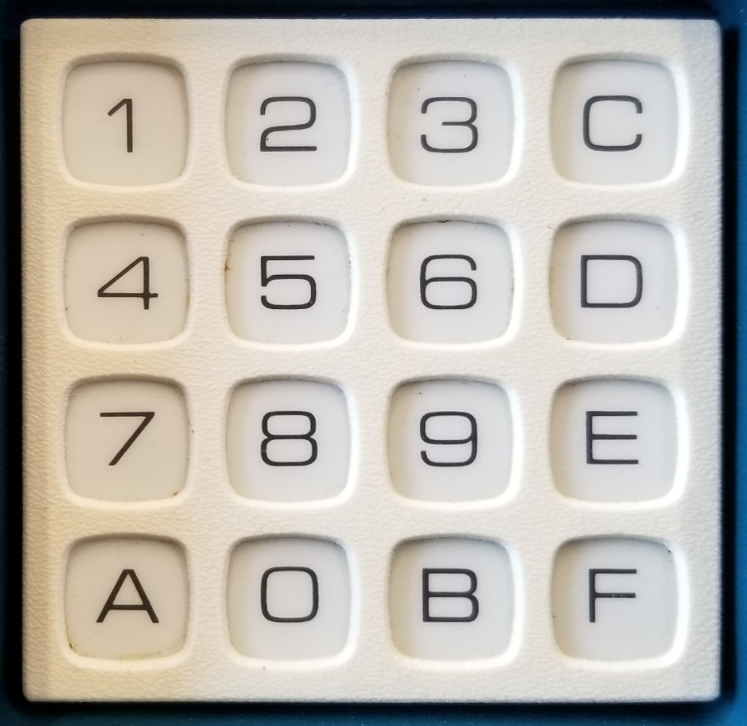
\includegraphics[width=0.6\textwidth]{figures/cosmac-vip-keypad.png}
	\end{center}
	\caption{Tastatura de pe COSMAC VIP}
	\label{fig:keypad}
\end{figure}

\section{Structura aplicației}
\subsection{Interpretarea \texttt{CHIP-8}}
\subsection{Extensia \texttt{SUPERCHIP}}
\subsection{Interfața grafică}

\section{Îmbunătățiri}

\section{Concluzii}

\newpage
\printbibliography[title=\section{Bibliografie}]

\renewcommand\listoflistingscaption{\section{Listinguri de cod sursă}}
\listoflistings

\end{document}
